\documentclass{article}
\usepackage[left=0.5in,top=0.5in,right=0.5in,bottom=0.5in]{geometry}
\usepackage[english]{babel}
\usepackage[utf8]{inputenc}
\usepackage[table]{xcolor}
\usepackage{amssymb,amsmath,amsthm}
\usepackage{changepage,threeparttable}
\usepackage{booktabs,multirow}
\usepackage{subcaption}
\usepackage{graphicx}
\usepackage{soul}
\graphicspath{{./images/}}
\def\F#1{\(#1\)}
\title{Lab 13: The DIY Inductor}
\author{Philip Kim}
\date{\today}
\begin{document}
\maketitle
\vspace*{-1cm}
\begin{table}[!htp]\centering
  \begin{tabular}{|c|c|}\hline
    \multicolumn{2}{|c|}{\textbf{Table 1: Sizes}}\\\hline
    Copper wire length \F{l}&51.2 cm\\\hline
    Diameter of pen \F{d}&0.25 cm\\\hline
    Number of windings \F{N}&70\\\hline
    Length of the inductor \F{a}&1.1 cm\\\hline
  \end{tabular}
\end{table}
\begin{table}[!htp]\centering
  \begin{tabular}{|c|c|c|c|c|c|c|}\hline
    \multicolumn{7}{|c|}{\textbf{Table 2: First Approximation for \F{R_{int}}}}\\\hline
    \F{f (Hz)}&s/DIV&\F{V_{RL} (V)}&V/DIV for \F{V_{RL}}&\F{V_{L} (V)}&V/DIV for \F{V_{L}}&\F{R_{int} (\Omega)}\\\hline
    1000&0.5ms&2.98V&0.5V&0.04V&0.5V&1.36\\\hline
  \end{tabular}
\end{table}
\begin{table}[!htp]\centering
  \begin{tabular}{|c|c|c|c|c|c|c|c|c|c|}\hline
    \multicolumn{10}{|c|}{\textbf{Table 2: First Approximation for \F{L}}}\\\hline
    \F{f (Hz)}&s/DIV&\F{V_{RL} (V)}&V/DIV for \F{V_{RL}}&\F{V_{L} (V)}&V/DIV for \F{V_{L}}&\F{I_R (A)}&\F{Z_{L,eff} (\Omega)}&\F{X_L (\Omega)}&L (H)\\\hline
    65000&20us&3.02V&0.5V&0.06V&0.5V&0.030&1.99&0.402&9.84e-7\\\hline
  \end{tabular}
\end{table}
\begin{table}[!htp]\centering
  \begin{tabular}{|c|c|c|c|c|c|}\hline
    \multicolumn{6}{|c|}{\textbf{Table 3: The Impedance of an Inductor}}\\\hline
    \F{f (Hz)}&s/DIV&\F{V_{RL} (V)}&V/DIV for \F{V_{RL}}&\F{V_{L} (V)}&V/DIV for \F{V_{L}}\\\hline
    1000&0.5ms&2.98V&0.5V&0.04V&0.5V\\\hline
    22000&20us&3.04V&0.5V&0.04V&0.5V\\\hline
    32000&20us&3.02V&0.5V&0.04V&0.5V\\\hline
    39000&20us&3.04V&0.5V&0.04V&0.5V\\\hline
    45000&20us&3.00V&0.5V&0.06V&0.5V\\\hline
    50000&20us&2.98V&0.5V&0.06V&0.5V\\\hline
    55000&20us&3.02V&0.5V&0.06V&0.5V\\\hline
    60000&20us&3.02V&0.5V&0.06V&0.5V\\\hline
    65000&20us&3.02V&0.5V&0.06V&0.5V\\\hline
  \end{tabular}
\end{table}
\begin{center}
  \subsection*{SETUP}
  \begin{figure}[!htp]
    \begin{subfigure}{0.5\textwidth}
    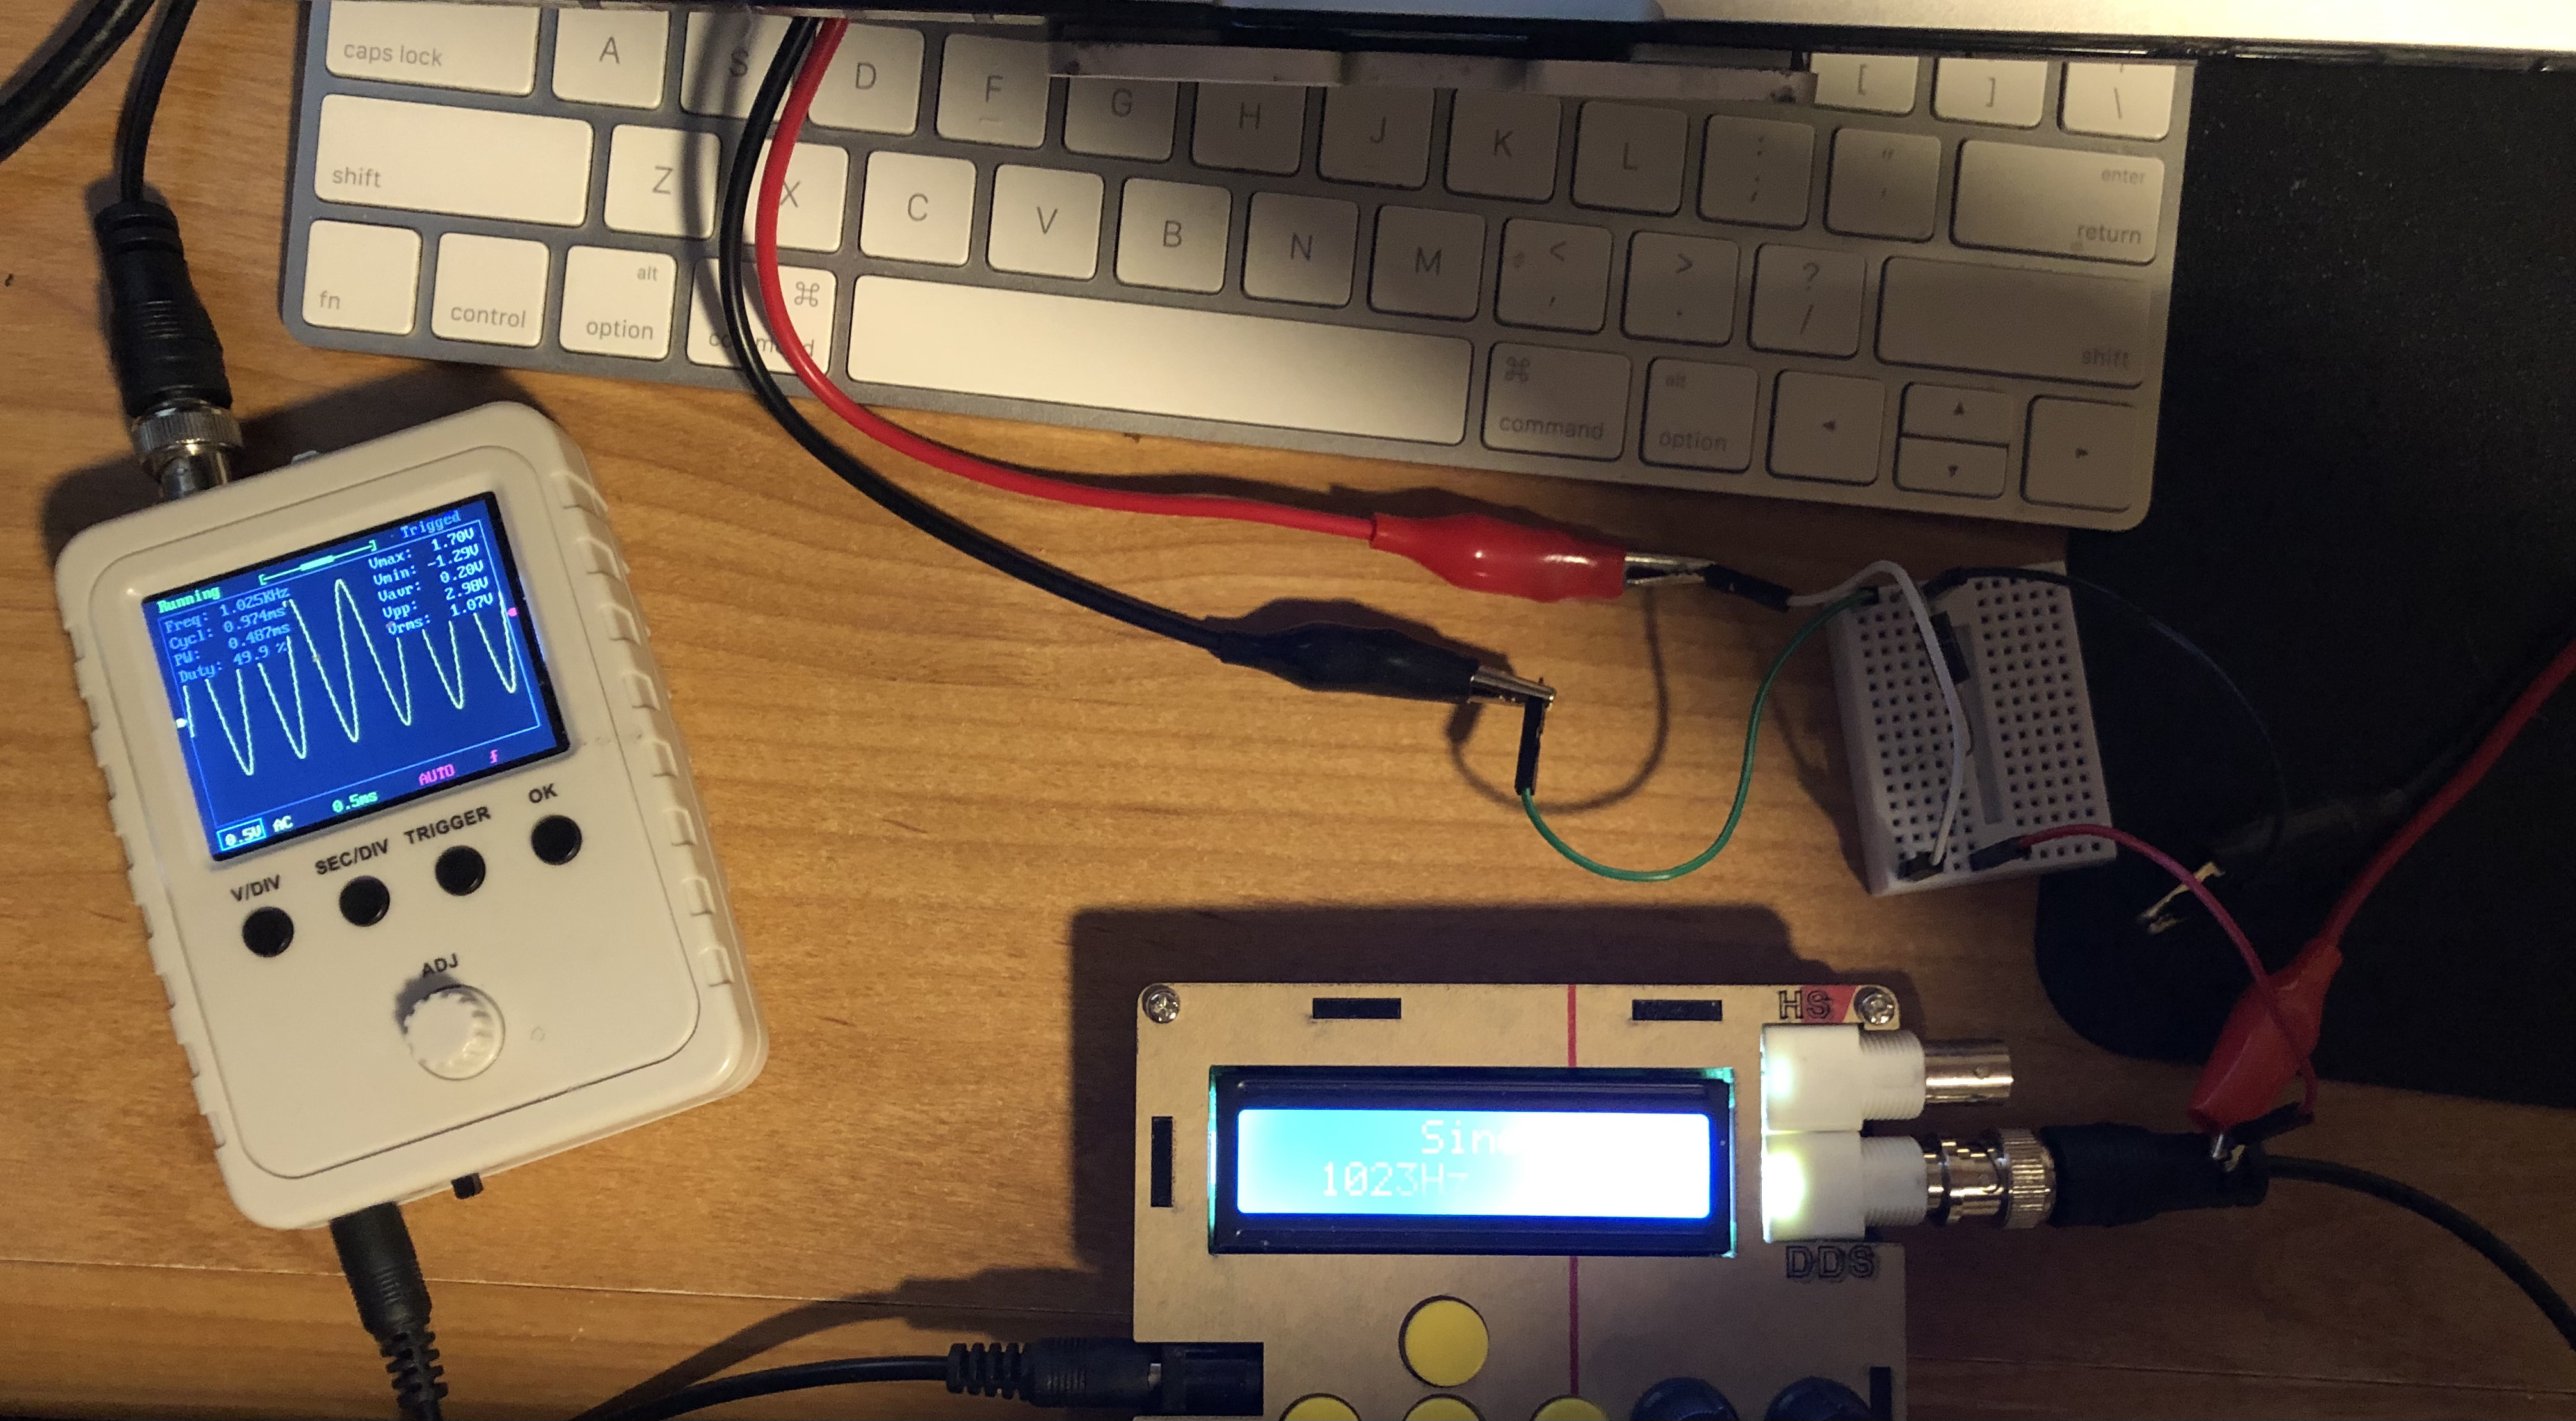
\includegraphics[scale=0.0665]{V_RL.jpeg}
    \caption*{\F{V_{RL}}}\label{fig:subim1}
    \end{subfigure}
    \begin{subfigure}{0.5\textwidth}
    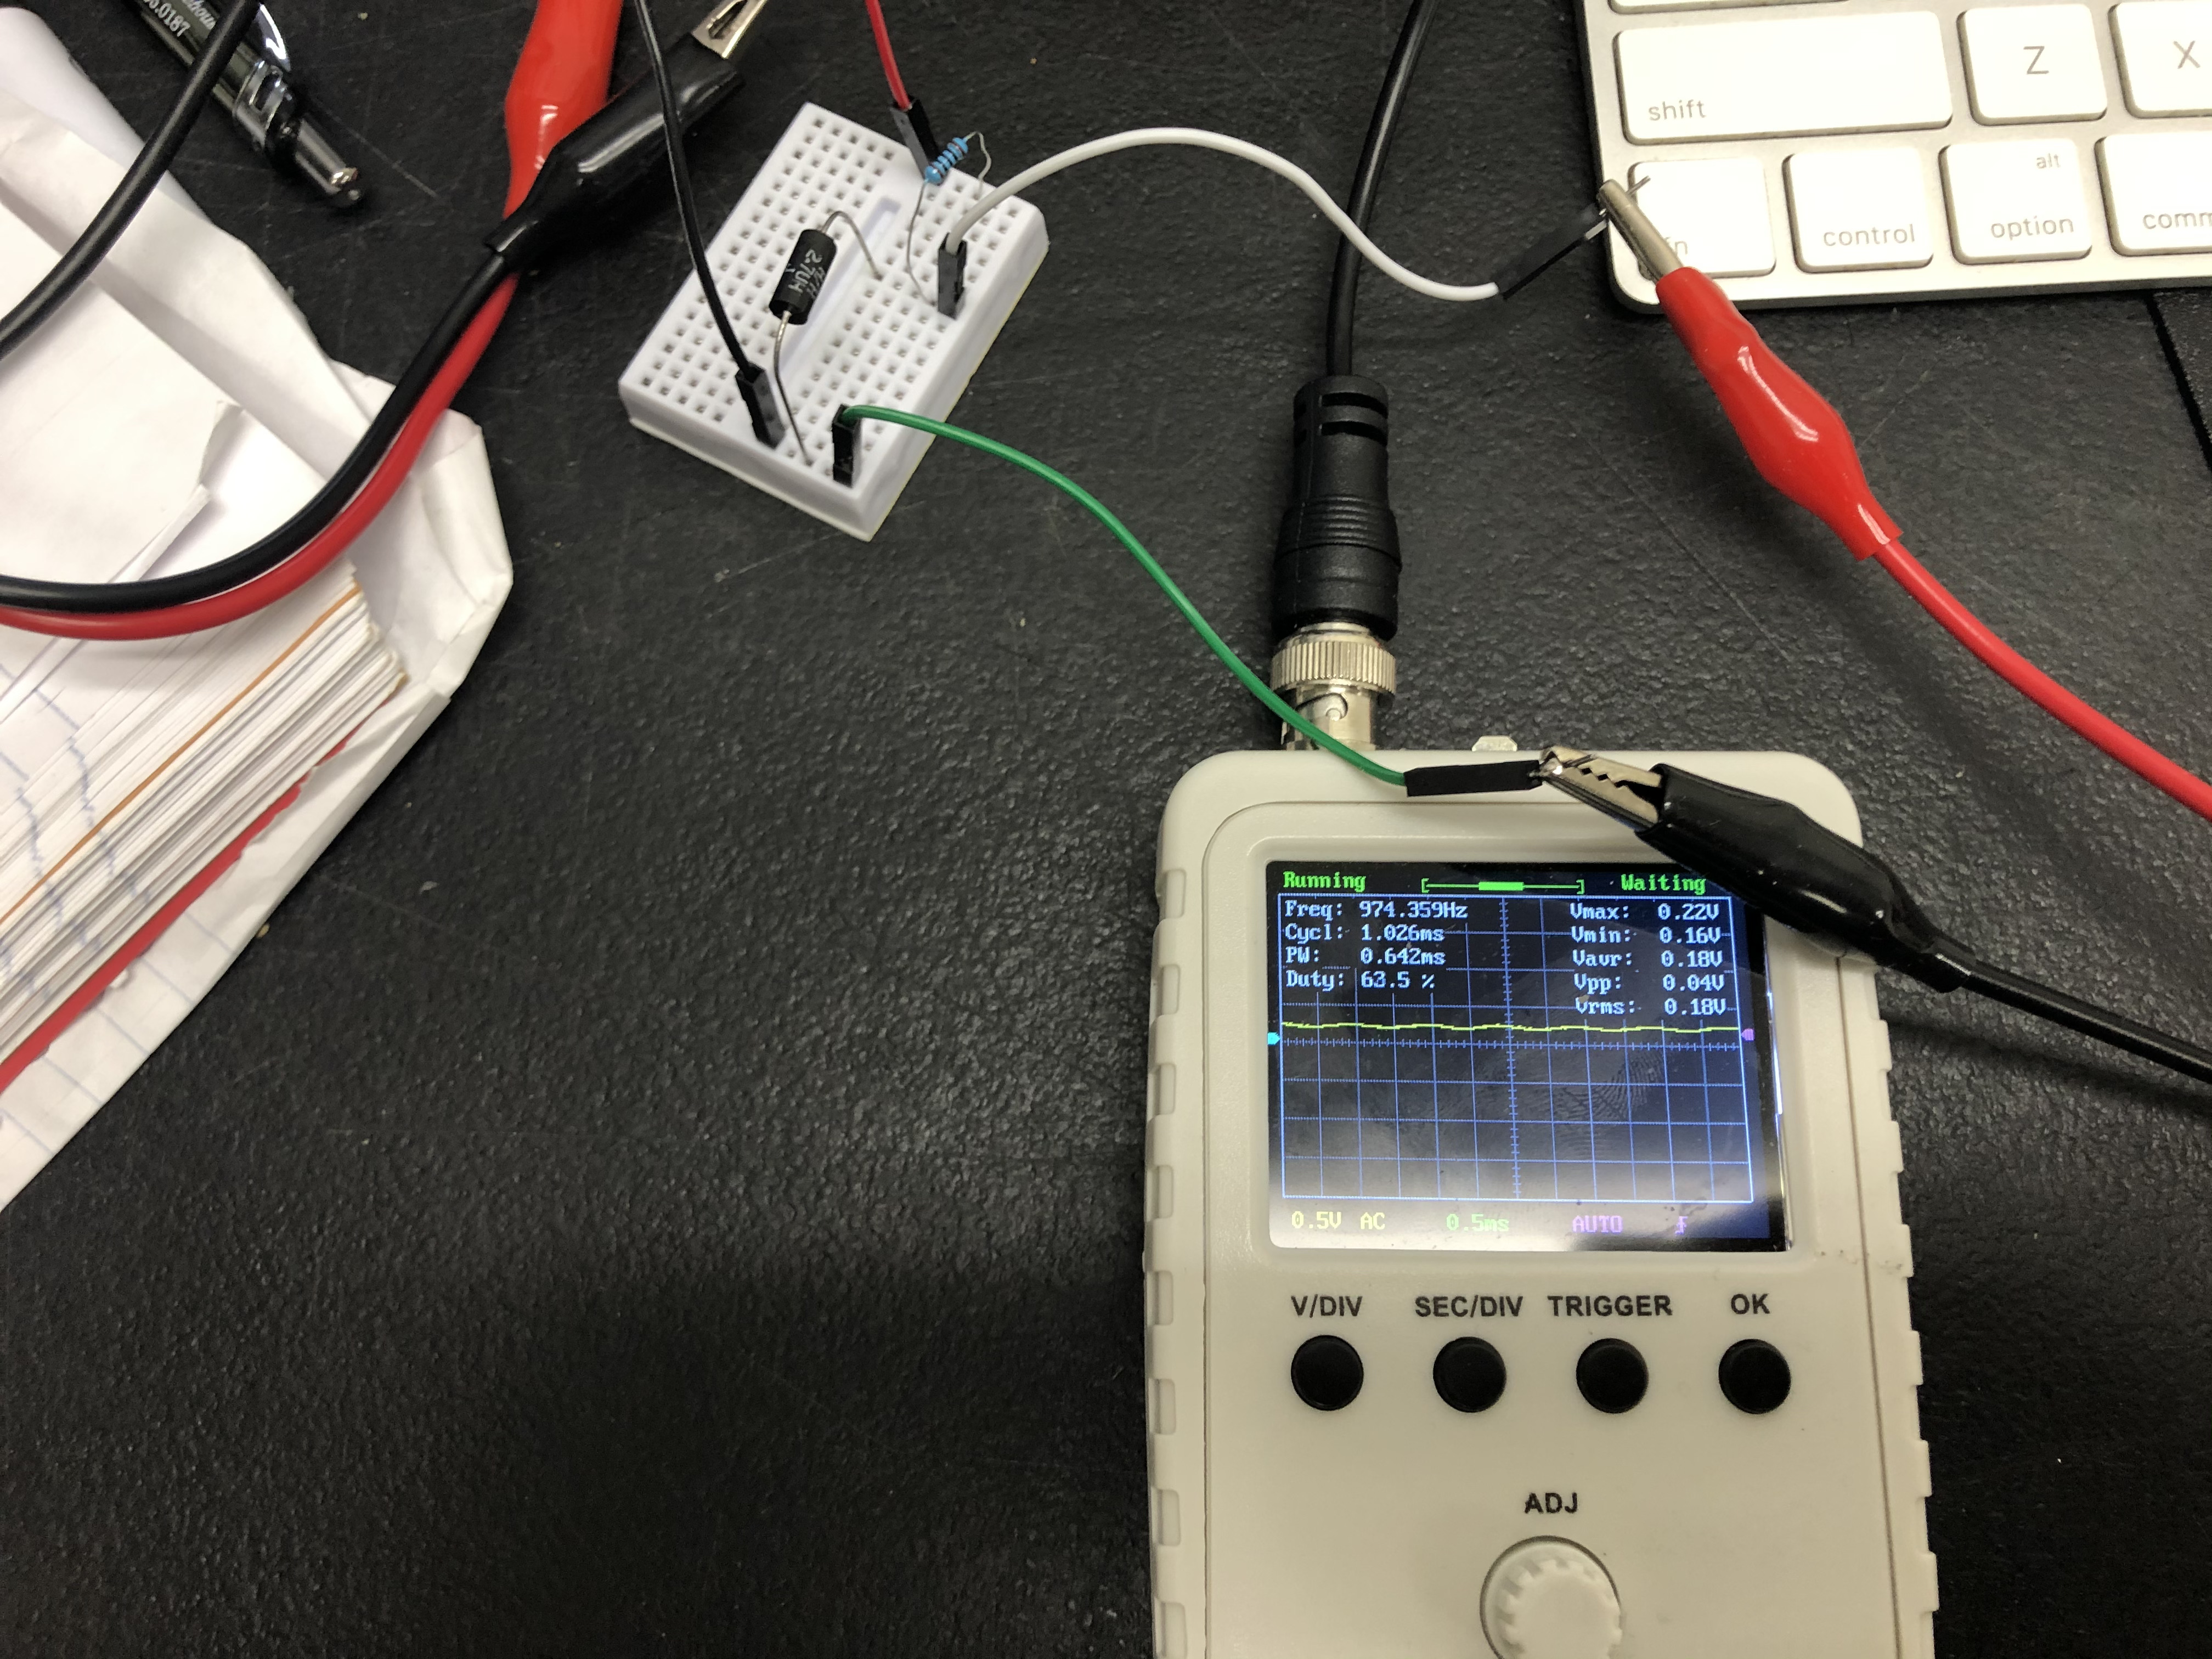
\includegraphics[scale=0.066]{V_L.jpeg}
    \caption*{\F{V_{L}}}\label{fig:subim2}
    \end{subfigure}
  \end{figure}
  \subsection*{GRAPH}
  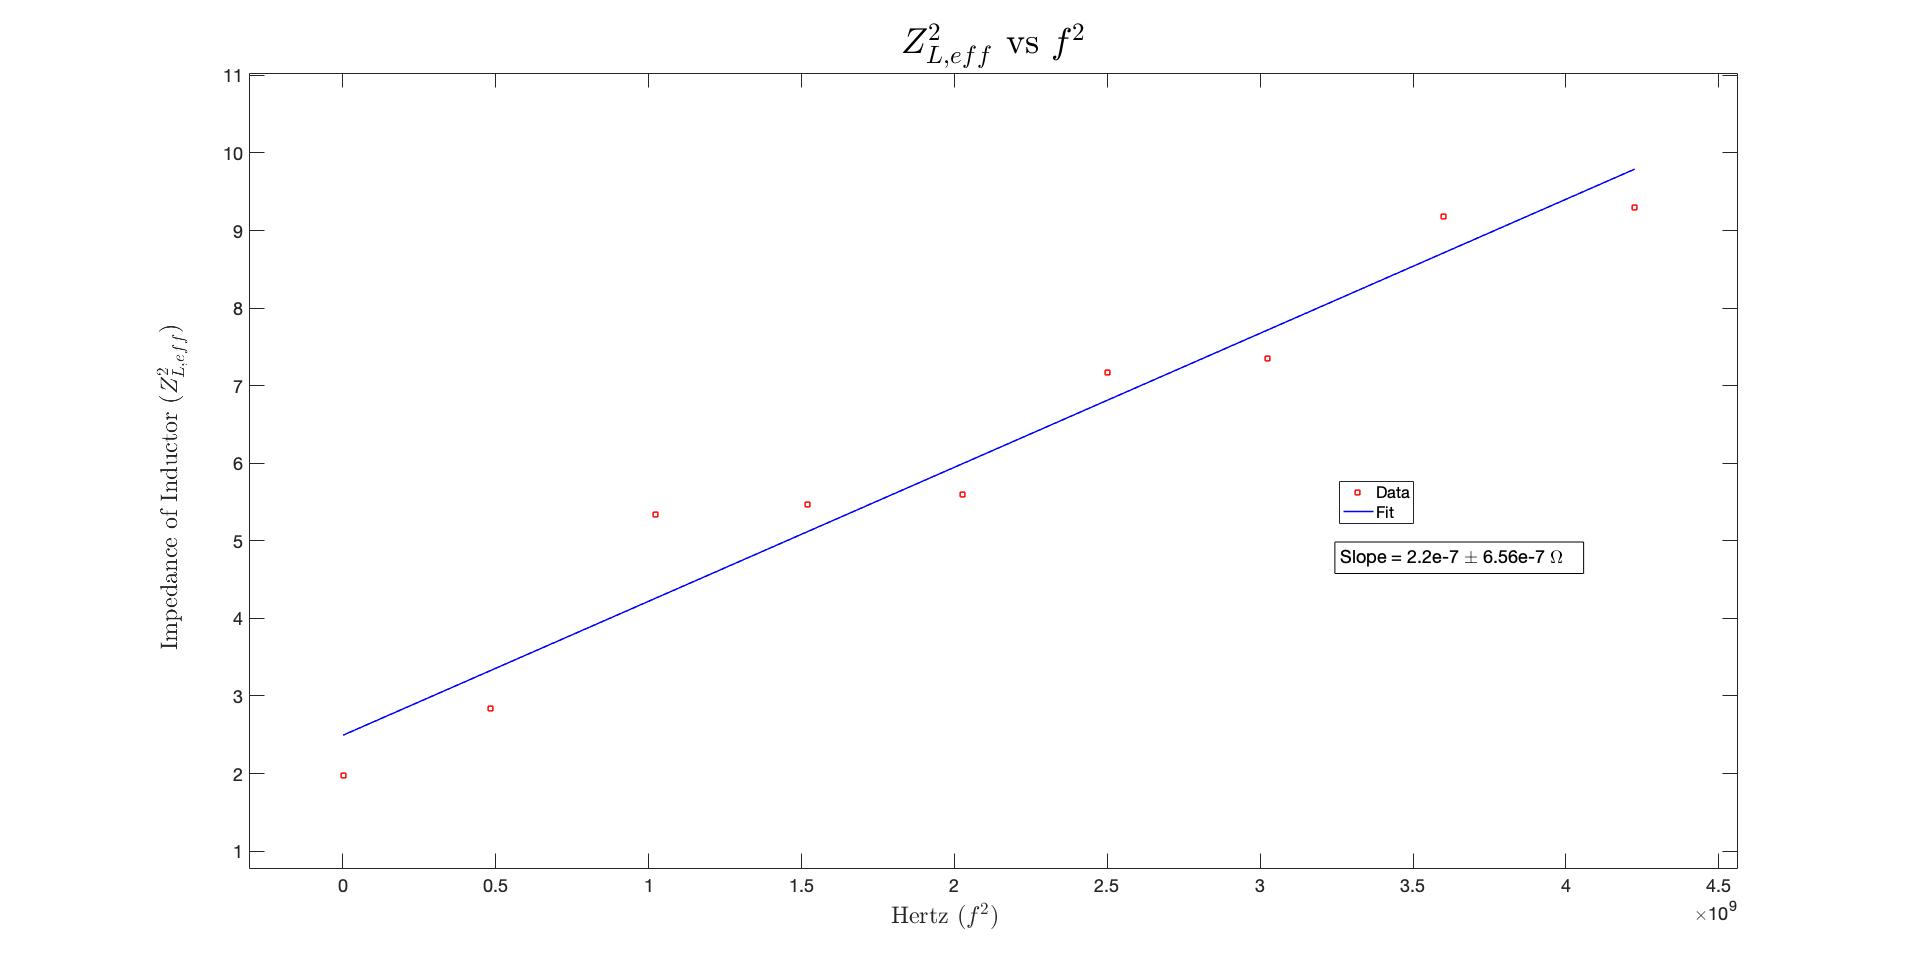
\includegraphics[width=\textwidth]{graph.jpg}
\end{center}
\begin{itemize}
  \item Compare the obtained value to that predicted for an ideal long inductor made of a wire of length l and taking up length a along the toothpick, \F{L=\frac{l^2}{a}\times{10}^{-7}H\rightarrow~L=\frac{.512 m}{.011 m}\times{10}^{-7}H\rightarrow~L=4.65\times{10}^{-7}H}
\end{itemize}
\end{document}
